% Monitoramento de servidores Linux por web sites.
%====================================================================================================
% TCC
%----------------------------------------------------------------------------------------------------
% Autor				    : Eduardo Balan
% Orientador		  : Kleber Krugrer
% Instituição 		: UFMS - Universidade Federal do Mato Grosso do Sul
% Departamento		: CPCX - Sistema de Informação
%----------------------------------------------------------------------------------------------------
% Data de criação	: 29 de Março de 2017
%====================================================================================================

\chapter{Desenvolvimento}\label{cap:Desenvolvimento}

Neste trabalho foi desenvolvido um sistema para monitoramento de servidores linux, utilizando a arquitetura cliente-servidor.
O sistema consiste em duas aplicações, uma desenvolvida em java que é um \textit{web service} para a qual foi dado o nome de \textbf{MonitorWeb-Api}. A outra aplicação em C++ que sera executada nos servidores linux cliente e tem o nome de \textbf{MonitorWeb-Cli}.

O MonitorWeb-Cli ira realizar leitura dos dados de seu hospedeiro tais como CPU(Central Processing Unit), memoria, banco dados e swap. Esse procedimento sera realizado de acordo com a configuração de tempo que o usuário desejar. Para cada leitura realizada o sistema realiza um envio dos dados para o MonitorWeb-Api. Ele também pode realizar rotinas de \textit{backups}(cópia de segurança) e \textit{vaccum}(Processo de limpeza no banco de dados) do banco dados PostgreSQL tanto no hospedeiro quanto em outro computador a qual ele tenha acesso pela rede. Após efetuar um desses procedimento ele também envia uma mensagem para o MonitorWeb-Api que por sua vez armazena essas informações.

O MonitorWeb-Api é responsável por receber os dados de todos os MonitorWeb-Cli, e realizar a persistência no banco de dados. Ele também pode ser utilizado para disponibilizar esse dados para outras aplicações.


%Como visto no capitulo \autoref{sec:ArquiteturaClienteServidor}, na arquitetura cliente-servidor, há um hospedeiro sempre em funcionamento denominado servidor, que atende a requisições de muitos outros hospedeiros. Para essa sistema foi dada nome de MonitorWeb-Api. Do outro lado dessa arquitetura temos os sistemas denominados clientes, e estes podem estar em funcionamento às vezes ou sempre. Para esse sistema foi dado o nome de MonitorWeb-Cli.

%Os dados monitorados são CPU (Central Processing Unit), memoria, swap e postgresql. Esses dados são lidos da maquina hospedeira cliente e enviado para o sistema servidor, que tem a função de receber e armazenar essas informações de forma persistente, para disponibiliza-las mais tarde.

\section{MonitorWeb-Api}\label{sec:MonitorWeb-Api}

O MonitorWeb-Api, é um \textit{web Service} desenvolvido utilizando a tecnologia Spring-boot, para o desenvolvimento de uma aplicação ReST que utiliza o protocolo HTTP/1.1 na comunicação com sistema clientes. A forma de passar dados entre os sistema foi utilizado o JSON (\textit{JavaScript Object Notation}) em vez do XML por ter sua estrutura menor e consumir menos trafego na rede \cite{Saudate:2014}. Para a persistência dos dados foi utilizado o banco de dados PostgreSQL.

O MonitorWeb-Api possui uma classe central chamado de Servidor. A partir do cadastro de um objeto dessa classe e o cadastro de um objeto da classe ServidorConfig e ambos estando relacionados, a aplicação já esta configurada para trabalhar com o MonitorWeb-Cli. Na \autoref{Tab:VariaveisServidor} e na \autoref{Tab:VariaveisServidorConfig} estão as variáveis e descrição das classe Servidor e ServidorConfig respectivamente. Como realizar o cadastro desses recursos sera mostrado na \autoref{subsec:ComsumindoRecursos}. 


% Please add the following required packages to your document preamble:
% \usepackage[table,xcdraw]{xcolor}
% If you use beamer only pass "xcolor=table" option, i.e. \documentclass[xcolor=table]{beamer}
\begin{table}[!ht]
\centering
\begin{tabular}{|l|l|}
\hline
{\color[HTML]{000000} \textbf{Variáveis}} & {\color[HTML]{000000} \textbf{Descriçães}}                                                                \\ \hline
id                                     & \multicolumn{1}{p{13.00cm}|}{Número único para cada objeto do tipo Servidor. (Gerado Automaticamente) }\\ \hline
dominio                                & \multicolumn{1}{p{13.00cm}|}{A qual domínio o servidor pertence (Não obrigatório)} \\ \hline
dthr\_cadastro                         & \multicolumn{1}{p{13.00cm}|}{Data e hora do cadastro. (Valor gerado automaticamente)} \\ \hline
nome                                   & \multicolumn{1}{p{13.00cm}|}{Nome que o usuário deseja dar ao servidor.}  \\ \hline
empresa                                & \multicolumn{1}{p{13.00cm}|}{Nome da empresa (Não obrigatório)} \\ \hline
observacao                             & \multicolumn{1}{p{13.00cm}|}{Alguma observação a fazer sobre o servidor (Não obrigatório)} \\ \hline
\end{tabular}
\caption[Variáveis da classe Servidor e suas descrições.]{Variáveis da classe Servidor e suas descrições.}
\label{Tab:VariaveisServidor}
\end{table}

% Please add the following required packages to your document preamble:
% \usepackage[table,xcdraw]{xcolor}
% If you use beamer only pass "xcolor=table" option, i.e. \documentclass[xcolor=table]{beamer}
\begin{table}[!ht]
\centering
\begin{tabular}{|l|l|}
\hline
{\color[HTML]{000000} \textbf{Variáveis}} & {\color[HTML]{000000} \textbf{Descriçães}} \\ \hline
id                                     & \multicolumn{1}{p{10.00cm}|}{Número único para cada objeto do tipo ServidorConfig. (Gerado Automaticamente)} \\ \hline
servidor                               & \multicolumn{1}{p{10.00cm}|}{Indica com qual servidor esse registro esta relacionado.}
\\ \hline
dthr\_cadastro                         & \multicolumn{1}{p{10.00cm}|}{Data e hora do cadastro. (Gerado Automaticamente)}\\ \hline
dthr\_alteracao                        & \multicolumn{1}{p{10.00cm}|}{Data e hora que foi realizado a ultima alteração. (Gerado Automaticamente)}\\ \hline
intervaloLeituraConfiguracoes          & \multicolumn{1}{p{10.00cm}|}{De quantos em quantos segundos o MonitorWeb-Cli deve ler esse arquivo de configurações, e se reconfigurar(Valor \textit{default} 120 s).} \\ \hline
intervaloLeituraConfiguracoesDb        & \multicolumn{1}{p{10.00cm}|}{De quantos em quantos segundos o MonitorWeb-Cli deve ler as configurações do banco de dados, e se reconfigurar(Valor \textit{default} 120 s).} \\ \hline
intervaloCpu                           & \multicolumn{1}{p{10.00cm}|}{De quantos em quantos segundos o MonitorWeb-Cli deve enviar um registro da classe MonitoramentoCpu.(Valor \textit{default} 1 s)}\\ \hline
intervaloMemoria                       & \multicolumn{1}{p{10.00cm}|}{De quantos em quantos segundos o MonitorWeb-Cli deve enviar um registro da classe MonitoramentoMemoria.(Valor \textit{default} 1 s)}\\ \hline
intervaloSwap                          & \multicolumn{1}{p{10.00cm}|}{De quantos em quantos segundos o MonitorWeb-Cli deve enviar um registro da classe MonitoramentoSwap.(Valor \textit{default} 1 s)} \\ \hline
hostMonitoramento                      & \multicolumn{1}{p{10.00cm}|}{IP do servidor principal do MonitorWeb-Api.}\\ \hline
hostMonitoramento2                     & \multicolumn{1}{p{10.00cm}|}{IP do servidor secundario do MonitorWeb-Api.} \\ \hline
porta                                  & \multicolumn{1}{p{10.00cm}|}{Porta da aplicação no servidor principal do MonitorWeb-Api.} \\ \hline
porta2                                 & \multicolumn{1}{p{10.00cm}|}{Porta da aplicação no servidor secundario do MonitorWeb-Api.} \\ \hline
\end{tabular}
\caption[Variáveis da classe ServidorConfig e suas descrições.]{Variáveis da classe ServidorConfig e suas descrições.}
\label{Tab:VariaveisServidorConfig}
\end{table}

Um diagrama de classe resumido pode ser visto na \autoref{Img:DiagramaDeClassResumidoDoResumo} contendo as duas classes citadas anteriormente, e diversos outros recursos que estão separados por cores. A seguir uma listagem falando sobre cada bloco de cor do diagrama. 


\begin{itemize}
		\item No quadro amarelo (classes com prefixo Servidor) corresponde as classes que o usuário tem que cadastrar para os recursos funcionarem.
		por exemplo para um monitoramento ocorrer um objeto da classe "ServidorConfig" deve ser criado e relacionado com o objeto da classe servidor em questão.
		\item No quadro rosa (classes com prefixo Informacoes) são classes que serão cadastradas automaticamente pela aplicação MonitorWeb-Cli e fazem referencia a os valores do servidor que são inseridos a cade vez que a aplicação é iniciada. Esses tipos de valores não tem como ser mudado sem que a maquina seja reiniciada. Um exemplos desses valor é o modelo do processador, ele nunca sera mudado sem que a maquina seja reiniciada.
		\item No quadro laranja (classes com prefixo Monitoramento) são classes que contem valores que precisam ser monitorados de tempos em tempo. Os intervalos de tempo do monitoramento das classe MonitoramentoCpu, MonitoramentoMemoria e MonitoramentoSwap são configurado através do objeto "ServidorConfig" como pode ser visto pela \autoref{Tab:VariaveisServidorConfig}. Exemplos dos valores armazenados por objetos dessa classe são quanto de memoria esta sendo utilizado e quantos Mhz cada núcleo do processador esta utilizado.
\end{itemize}


\begin{figure}[H]
	\centering
	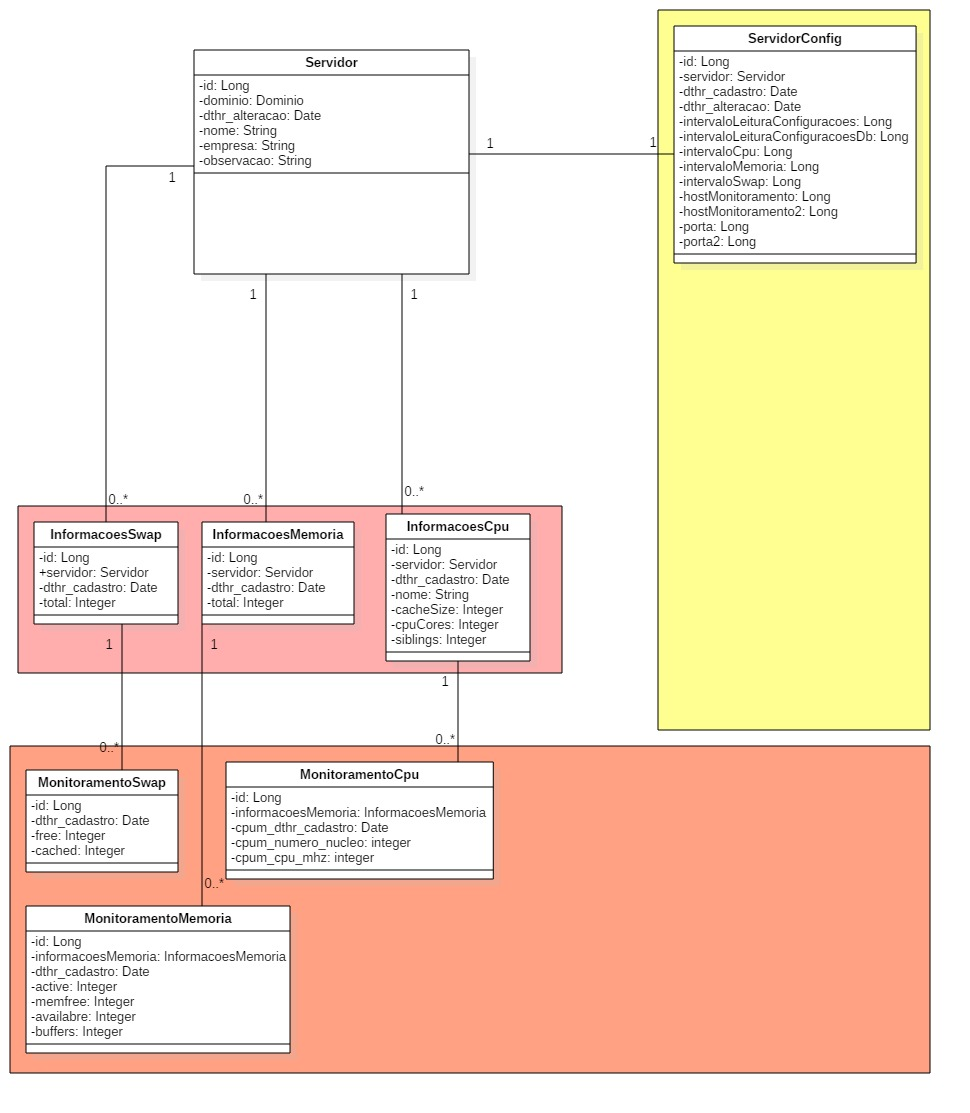
\includegraphics[width=1.0\textwidth]{figuras/DiagramaDeClassResumidoDoResumo.jpg}
	\caption[Diagrama de classe resumido 1.]{Diagrama de classe resumido 1, separados pelas cores amarelo, rosa e laranja que correspondem respectivamente a configurações que o usuário deve fazer, informações geradas pelo MonitorWeb-Api e monitoramentos gerados pelo MonitorWeb-Api}
	\label{Img:DiagramaDeClassResumidoDoResumo}
	
	%width=0.5\textwidth (Tamanho da Imagem)
\end{figure}






\begin{figure}[H]
	\centering
	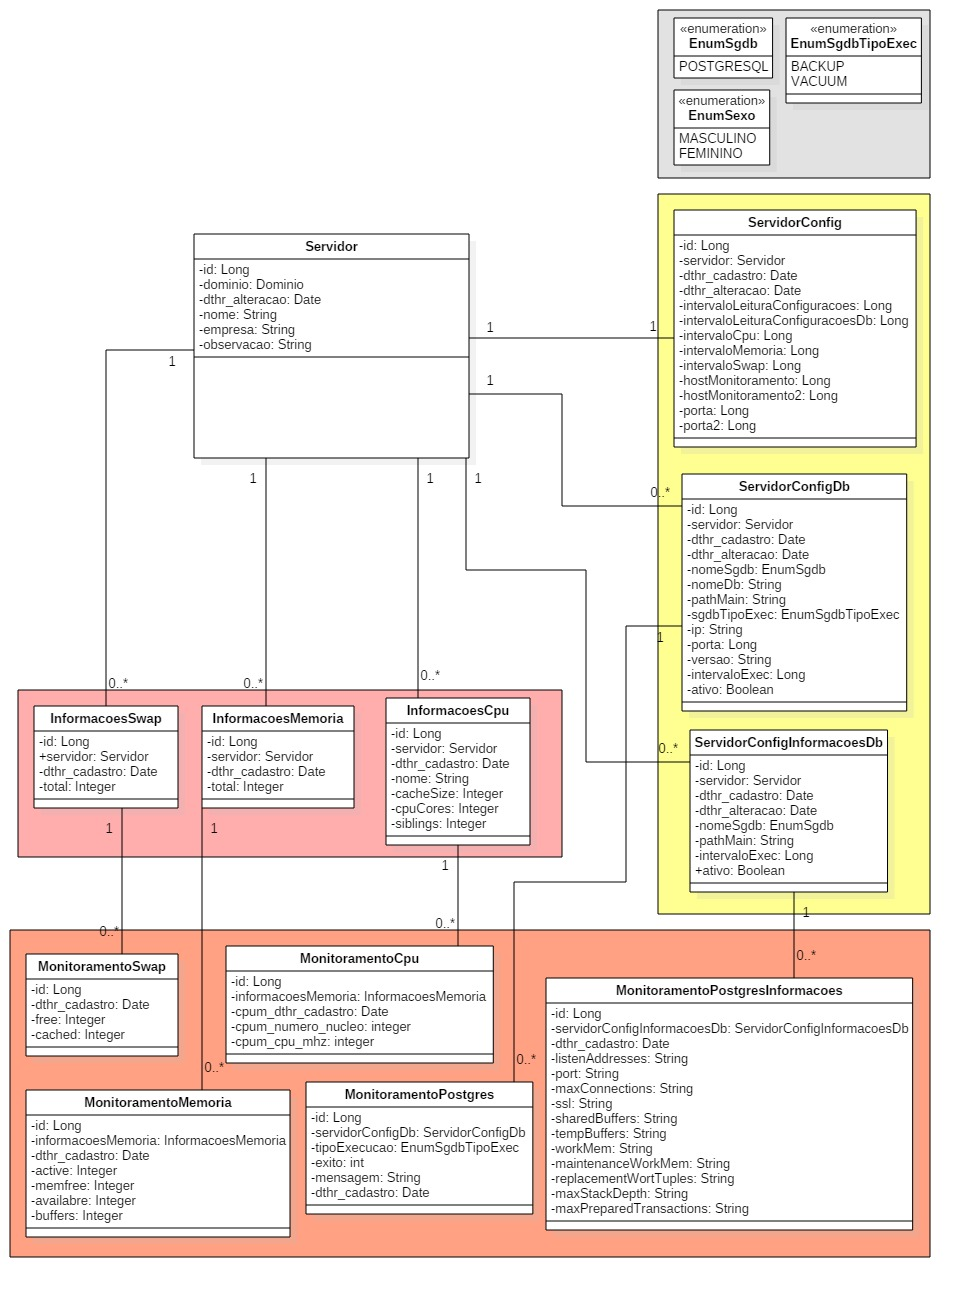
\includegraphics[width=1.0\textwidth]{figuras/DiagramaDeClassResumido.jpg}
	\caption[Diagrama de classe resumido 2.]{Diagrama de classe resumido 2, separados pelas cores amarelo, rosa e laranja que correspondem respectivamente a configurações que o usuário deve fazer, informações geradas pelo MonitorWeb-Api e monitoramentos gerados pelo MonitorWeb-Api}
	\label{Img:estruturaDePastaPojetoEntity}
	
	%width=0.5\textwidth (Tamanho da Imagem)
\end{figure}












\subsection{Configurações Apache Maven}\label{subsec:ConfiguraçõesApacheMaven}

Como visto na \autoref{sec:ApacheMaven} o Apache Maven é um gerenciador de pacotes, que gerenciá as dependências por meio do arquivo POM.
Esse arquivo pode ser encontrado na raiz do projeto /pom.xml.
No \autoref{Func:POMMonitorWebApi}, é mostrado as principais dependências contidas nesse arquivo, a seguir é explicado cada uma das dependências.

\begin{itemize}\label{List:Pom}
		\item \autoref{Func:POMMonitorWebApi}, linha 3 - spring-boot-starter-parent, Dependência do Spring-boot. Ele também cria um "parent" que faz com que não seja necessário especificar as versões nos outros pacotes do spring, pois ele já identificara a versão automaticamente \cite{springBoot:2017}.
		
		\item \autoref{Func:POMMonitorWebApi}, linha 10 - spring-boot-starter-data-jpa, Dependência que spring-data-jpa. Ele traz automaticamente todas as dependencias necessarias para o seu funcionamento \cite{springDataJpa:2017}.
		
		\item \autoref{Func:POMMonitorWebApi}, linha 15 - spring-boot-starter-web, Essa dependência identifica que nossa aplicação sera uma aplicação \textit{web}, rodara usando tomcat, utilizara ReSTfull, seguindo padrão spring MVC(\textit{Model View Controller}) \cite{springBoot:2017}.
		
		\item \autoref{Func:POMMonitorWebApi}, linha 20 - spring-boot-starter-logging, Dependência responsável pelo registro de log automático \cite{springBoot:2017}.
		
		\item \autoref{Func:POMMonitorWebApi}, linha 25 - spring-boot-starter-test, Dependência do Spring Boot com bibliotecas de teste unitário, incluindo JUnit, Hamcrest e Mockito \cite{springBoot:2017}.
		
		\item \autoref{Func:POMMonitorWebApi}, linha 31 - postgresql, Dependência que fornece um conjunto padrão de interfaces para bancos de dados compatíveis com SQL \cite{PostgreSQL:2017}.
	
\end{itemize}


\begin{lstlisting}[style=XML,label=Func:POMMonitorWebApi,caption={[Arquivo POM com as principais dependências do projeto.]Arquivo POM com as principais dependências do projeto.}]
	<parent>
			<groupId>org.springframework.boot</groupId>
			<artifactId>spring-boot-starter-parent</artifactId>
			<version>1.3.3.RELEASE</version>
			<relativePath/>
	</parent>
	
	<dependency>
		<groupId>org.springframework.boot</groupId>
		<artifactId>spring-boot-starter-data-jpa</artifactId>
	</dependency>
	
	<dependency>
		<groupId>org.springframework.boot</groupId>
		<artifactId>spring-boot-starter-web</artifactId>
	</dependency>

	<dependency>
		<groupId>org.springframework.boot</groupId>
		<artifactId>spring-boot-starter-logging</artifactId>
	</dependency>

	<dependency>
		<groupId>org.springframework.boot</groupId>
		<artifactId>spring-boot-starter-test</artifactId>
		<scope>test</scope>
	</dependency>
				
	<dependency>
		<groupId>org.postgresql</groupId>
		<artifactId>postgresql</artifactId>
		<version>${postgresql.version}</version>
	</dependency>

	<dependency>
		<groupId>com.github.springtestdbunit</groupId>
		<artifactId>spring-test-dbunit</artifactId>
		<version>${spring-test-dbunit.version}</version>
		<scope>test</scope>
	</dependency>

	<dependency>
		<groupId>com.h2database</groupId>
		<artifactId>h2</artifactId>
		<scope>test</scope>
	</dependency>
\end{lstlisting}



\subsection{Configurações application.properties}\label{subsec:ConfiguraçõesApplicationProperties}

O spring fornece um arquivo de configuração com o nome de "application.properties", e pode ser encontrado na pasta /src/main/resources/application.properties. Dentro desse arquivo pode ser feitas configurações de acordo com a necessidade do projeto \cite{springBoot:2017}.

\begin{itemize}
		\item \autoref{Func:applicationProperties} linha 2, server.port - Porta que a aplicação ira rodar \cite{springBoot:2017}.
		
		\item \autoref{Func:applicationProperties} linha 5, spring.jackson.date-format -  Formato que a data sera apresentada \cite{springBoot:2017}.
		
		\item \autoref{Func:applicationProperties} linha 10, logging.path - Indica o local que ficara o arquivo de \textit{log} \cite{springBoot:2017}.
		
		\item \autoref{Func:applicationProperties} linha 11 a 14, logging.level.* - Indique se aquele nivel do spring tera o log ativado ou não.
		Alguns dos valores que eles podem receber são \textit{TRACE, DEBUG, INFO, WARN, ERROR, FATAL,} ou \textit{OFF} \cite{springBoot:2017}.
		
		\item \autoref{Func:applicationProperties} linha 19, spring.datasource.url - URL de conexão para o banco de dados \cite{springBoot:2017}.
		
		\item \autoref{Func:applicationProperties} linha 20, spring.datasource.username  - Usuario do banco de dados \cite{springBoot:2017}.
		
		\item \autoref{Func:applicationProperties} linha 21, spring.datasource.password  - Senha do banco de dados \cite{springBoot:2017}.
		
		\item \autoref{Func:applicationProperties} linha 22, spring.jpa.database-platform -  Vários bancos de dados têm mais de um \textit{Dialect}, e essa propriedade especifica que dialeto do hibernate ira utilizar \cite{springBoot:2017}.
		
		\item \autoref{Func:applicationProperties} linha 23, spring.datasource.driverClassName -  Nome do \textit{driver} que sera utilizado para conexão \cite{springBoot:2017}.
		
\end{itemize}

\begin{lstlisting}[style=LIVRE, label=Func:applicationProperties,caption={[Arquivo application.properties com as principais configurações do projeto.]Arquivo application.properties com as principais configurações do projeto.}]
## Portas
server.port=8081

## Formatador de datas do jackson
spring.jackson.date-format= yyyy-MM-dd'T'HH:mm:ss.SSSZ

## --------------------------------------------------------------------
## LOGGING
## --------------------------------------------------------------------
logging.path=../
logging.level.root=INFO
logging.level.org.hibernate = INFO
logging.level.org.springframework.web = INFO
logging.level.org.camunda=INFO

## --------------------------------------------------------------------
## POSTGRES
## --------------------------------------------------------------------
spring.datasource.url=jdbc:postgresql://localhost/webmonitor
spring.datasource.username=postgres
spring.datasource.password=postgres
spring.jpa.database-platform=org.hibernate.dialect.PostgreSQLDialect
spring.datasource.driverClassName=org.postgresql.Driver

\end{lstlisting}




\subsection{Estrutura do Projeto}\label{subsec:EstruturaDoProjeto}

O projeto foi dividido em seis pastas que podem ser visto na \autoref{Img:estruturaDePastaPojeto}, e uma classe chama WebMonitorApp.class, a qual é responsável por iniciar a aplicação. A \autoref{Tab:DescricaoDasPastasProjeto} temos o nome das pastas e suas descrição.



\begin{figure}[H]
	\centering
	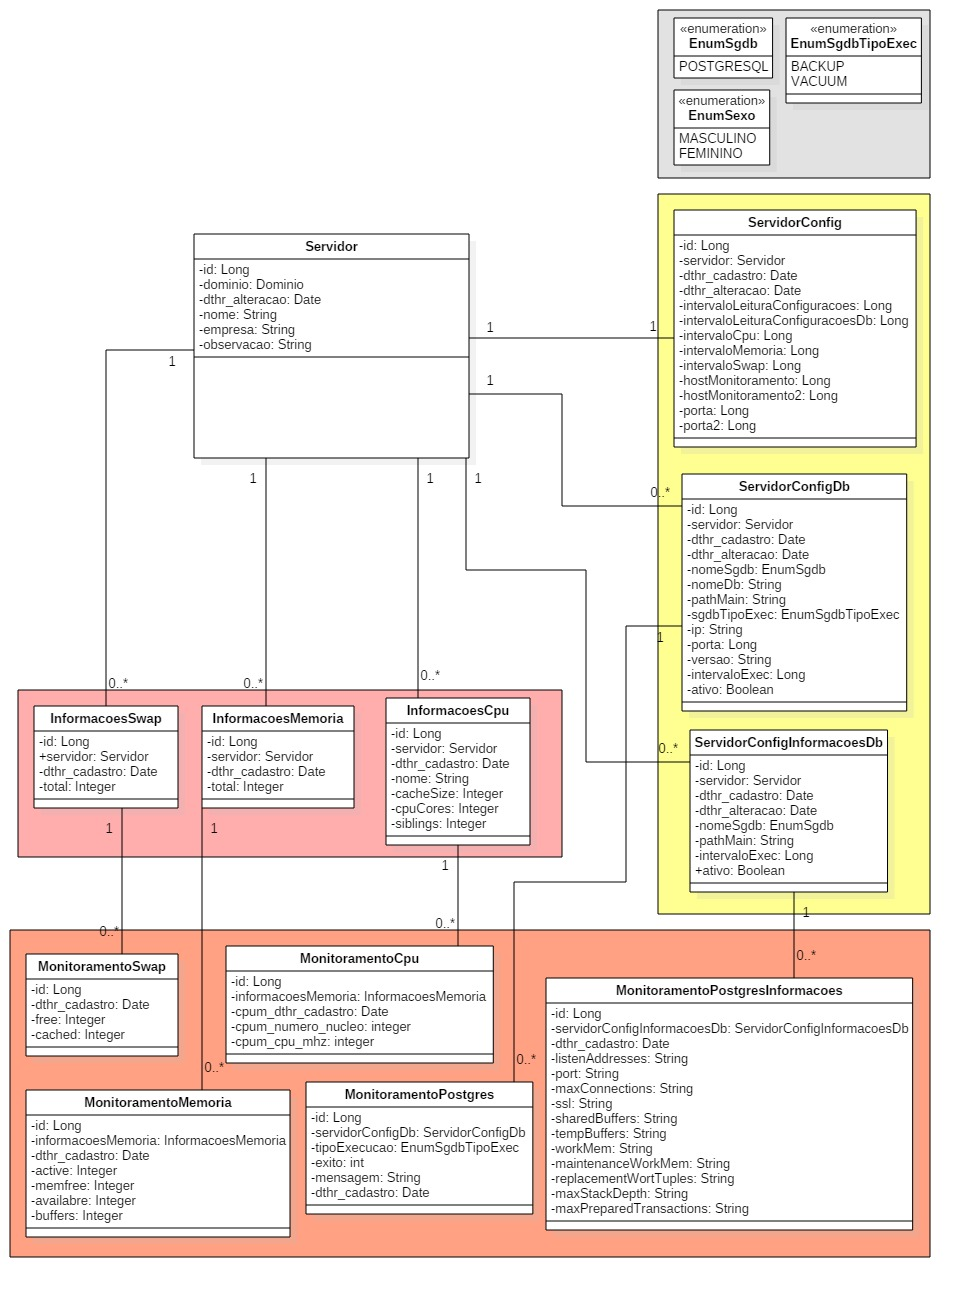
\includegraphics[width=1.0\textwidth]{figuras/DiagramaDeClassResumido.jpg}
	\caption[Pasta DiagramaDeClass.]{Pasta DiagramaDeClass.}
	\label{Img:estruturaDePastaPojetoEntity}
	
	%width=0.5\textwidth (Tamanho da Imagem)
\end{figure}

\begin{figure}[H]
	\centering
	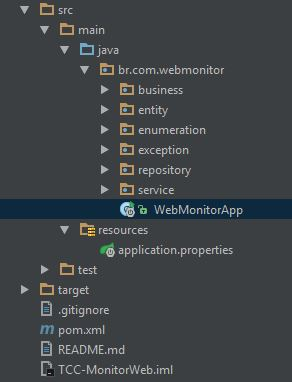
\includegraphics[width=0.4\textwidth]{figuras/estruturaPojeto.JPG}
	\caption[Estrutura de pastas do projeto.]{Estrutura de pastas do projeto.}
	\label{Img:estruturaDePastaPojeto}
	
	%width=0.5\textwidth (Tamanho da Imagem)
\end{figure}
	
% Please add the following required packages to your document preamble:
% \usepackage[table,xcdraw]{xcolor}
% If you use beamer only pass "xcolor=table" option, i.e. \documentclass[xcolor=table]{beamer}
\begin{table}[!ht]
\centering
\begin{tabular}{|l|l|}
\hline
\multicolumn{1}{|c|}{{\color[HTML]{000000} \textbf{Pasta}}} & \multicolumn{1}{c|}{{\color[HTML]{000000} \textbf{Descrição}}} \\ \hline
business                                                    & Responsavel pelas regras de negocio.                           \\ \hline
entity                                                      & Entidades do sistema.                                          \\ \hline
enumeration                                                 & Enum.                                                          \\ \hline
exception                                                   & Exception.                                                     \\ \hline
repository                                                  & Interfaces para gerar os acessos ao banco de dados.            \\ \hline
service                                                     & Responsáveis pelos serviços da aplicação.                      \\ \hline
\end{tabular}
\caption{Descrição das pastas do projeto.}
\label{Tab:DescricaoDasPastasProjeto}
\end{table}




\subsection{Pasta entity}\label{subsec:PastaEntity}

A paste entity é responsável pelas entidades da aplicação, e sua estrutura pode ser vistas na \autoref{Img:estruturaDePastaPojetoEntity}.
Os arquivos possuem três iniciais muito repetidas em seus nomes que são "Informacoes*", "Monitoramento*" e "ServidorConfig*" e cada uma delas possui um significado:

As classes que iniciam com a palavra "Informações", contem valores que só precisam ser armazenados uma única vez quando a aplicação é iniciada.
Esses tipos de valores não tem como ser mudado sem que a maquina seja reiniciada e o sistema de monitoramento cliente reinicie.
Exemplos desses valores são, modelo do processador, numero de núcleos do processador e quantidade de memoria.

As classes que iniciam com a palavra "Monitoramento*" contem valores que precisam ser armazenados de tempos em tempo, como quanto de memoria esta sendo utilizado, se o banco de dados executou o backup corretamente, quantos Mhz cada nucleo do processador esta endo utilizado.

As classes que iniciam com a palavra "ServidorConfig*" contem valores que o usuário deve configurar, como IP da aplicação, porta, tempo de intervalo de cada monitoramento.


\begin{figure}[H]
	\centering
	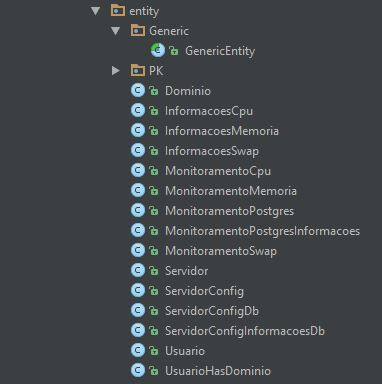
\includegraphics[width=0.4\textwidth]{figuras/estruturaPojetoEntity.JPG}
	\caption[Pasta Entity.]{Pasta Entity.}
	\label{Img:estruturaDePastaPojetoEntity}
	
	%width=0.5\textwidth (Tamanho da Imagem)
\end{figure}

\subsubsection{classe GenericEntity}\label{subsec:ClassGenericEntity}

Todas as entidades da aplicação estendem da classe abstrata GenericEntity que por sua vez recebe uma tipo <T> genérico que estende de Serializable.
Esse tipo <T> representa o tipo da variável ID da entidade, para que a aplicação saiba como gerar determinados métodos.
A classe GenericEntity pode ser vista no \autoref{Func:GenericEntity}
	
\begin{lstlisting}[style=Java, label=Func:GenericEntity,caption={[Entidade genérica da aplicação GenericEntity.]Entidade genérica da aplicação GenericEntity e suas funcionalidades.}]
package br.com.webmonitor.entity.Generic;

import java.io.Serializable;
import java.util.Date;
import java.util.Objects;

/**
 * Classe base para qualquer objeto serializável.
 *
 * @author Eduardo Balan
 *
 * @param <T> o tipo do atributo id
 */
public abstract class GenericEntity<T extends Serializable> implements Serializable {

    private static final long serialVersionUID = 1L;

    public abstract T getId();

    public abstract void setId(T id);

    public abstract Date getDthr_cadastro();

    public abstract void setDthr_cadastro(Date date);

    /**
     * Indica quando outro objeto é igual a este. Nesta implementação, qualquer objeto derivado de Bean é igual a este desde que seja exatamente da mesma classe e tenha o mesmo ID.
     *
     * @author Kleber Kruger
     *
     * @param obj o objeto a comparar com este
     * @return {@code true} se este objeto é igual ao do argumento; {@code false} caso contrário.
     */
    @Override
    public boolean equals(Object obj) {
        if (getId() != null && obj instanceof GenericEntity) {
            GenericEntity x = (GenericEntity) obj;
            return getClass() == x.getClass() && getId().equals(x.getId());
        }
        return super.equals(obj);
    }

    /**
     * Retorna um valor de hash code para este objeto. Nesta implementação, este valor é gerado por
     * uma combinação do hash code da classe (getClass().hashCode()) somado ao hash code do atributo
     * id (id.hashCode()).
     *
     * @author Kleber Kruger
     *
     * @return um valor de hash code para este objeto
     */
    @Override
    public int hashCode() {
        if (getId() != null) {
            return 43 * 7 + Objects.hashCode(getClass().hashCode() + getId().hashCode());
        }
        return super.hashCode();
    }

}
\end{lstlisting}


\subsection{Comsumindo recursos do MonitorWeb-Api}\label{subsec:ComsumindoRecursos}

\section{MonitorWeb-Cli}\label{sec:MonitorWeb-Cli}

\begin{figure}[H]
	\centering
	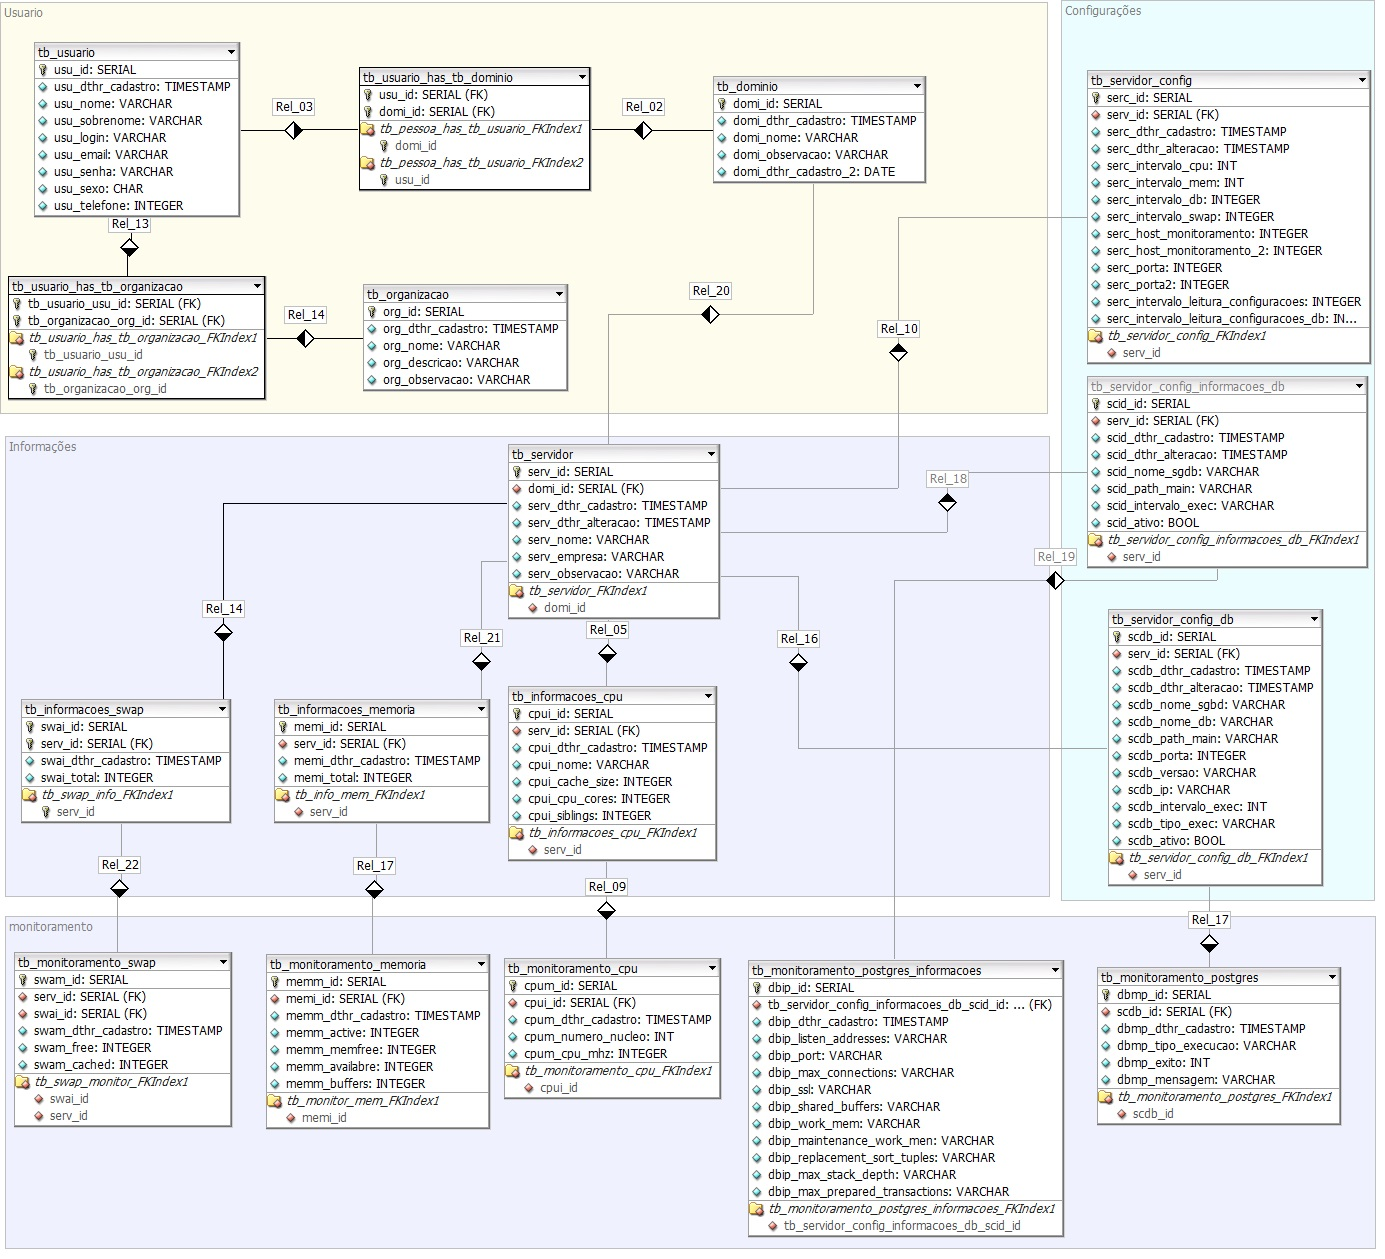
\includegraphics[width=1.0\textwidth]{figuras/diagramaBanco.jpg}
	\caption[Pasta Entitybbbbbbbbbbbbbbbbbbbbbbbbbbbbbbbbbb.]{Pasta Entityaaaaaaaaaaaaaaaaaaaaaaaaaaaaaaaaaaaa.}
	\label{Img:estruturaDePastaPojetoEntity}
	
	%width=0.5\textwidth (Tamanho da Imagem)
\end{figure}


